\documentclass{article}
\usepackage{graphicx}
\graphicspath{ {./images/} }
\usepackage{amsmath}

\title{4. Determinanti. Matricu reizināšana}
\author{Gunārs Ābeltiņš}
\date{2022.03.12}

\begin{document}

\maketitle

\section*{Lekcijas konspekts}
Matricu īpašibas. Kad drīkts reizināt. Efektīva determinanta aprēķināšana.

\clearpage

\section*{1. Uzdevums}
Izmantojot Gausa metodi (ne savādāk), aprēķiniet determinantu Det [\{2,3,5,2\}, \{1,3,3,0\}, \{2,1,2,0\},\{2,0,1,5\}] . Mēģiniet pārkārtot rindas un/vai kolonnas, lai ietaupītu darbības. Rezultātu pārbaudiet ar WolframAlpha.

\begin{gather*}
    \det
    \begin{pmatrix}
        2 & 3 & 5 & 2\\
        1 & 3 & 3 & 0\\
        2 & 1 & 2 & 0\\
        2 & 0 & 1 & 5
    \end{pmatrix} 
    =
    \begin{vmatrix}
        2 & 3 & 5 & 2\\
        1 & 3 & 3 & 0\\
        2 & 1 & 2 & 0\\
        2 & 0 & 1 & 5
    \end{vmatrix}
    =
    -
    \begin{vmatrix}
        1 & 3 & 3 & 0\\
        2 & 3 & 5 & 2\\
        2 & 1 & 2 & 0\\
        2 & 0 & 1 & 5
    \end{vmatrix}
    =
    \\
    =
    -
    \begin{vmatrix}
        1 & 3 & 3 & 0\\
        0 & -3 & -1 & 2\\
        0 & 1 & 1 & -5\\
        0 & -6 & 5 & 5
    \end{vmatrix}
    =
    \begin{vmatrix}
        1 & 3 & 3 & 0\\
        0 & 1 & 1 & -5\\
        0 & -3 & -1 & 2\\
        0 & -6 & 5 & 5
    \end{vmatrix}
    =
    \begin{vmatrix}
        1 & 3 & 3 & 0\\
        0 & 1 & 1 & -5\\
        0 & 0 & 2 & -13\\
        0 & 0 & 1 & -25
    \end{vmatrix}
    =
    \\
    =
    -
    \begin{vmatrix}
        1 & 3 & 3 & 0\\
        0 & 1 & 1 & -5\\
        0 & 0 & 1 & -25\\
        0 & 0 & 2 & -13
    \end{vmatrix}
    =
    -
    \begin{vmatrix}
        1 & 3 & 3 & 0\\
        0 & 1 & 1 & -5\\
        0 & 0 & 1 & -25\\
        0 & 0 & 0 & 37
    \end{vmatrix}
    =
    -(1 \cdot 1 \cdot 1 \cdot 37)
    =
    -37
\end{gather*}

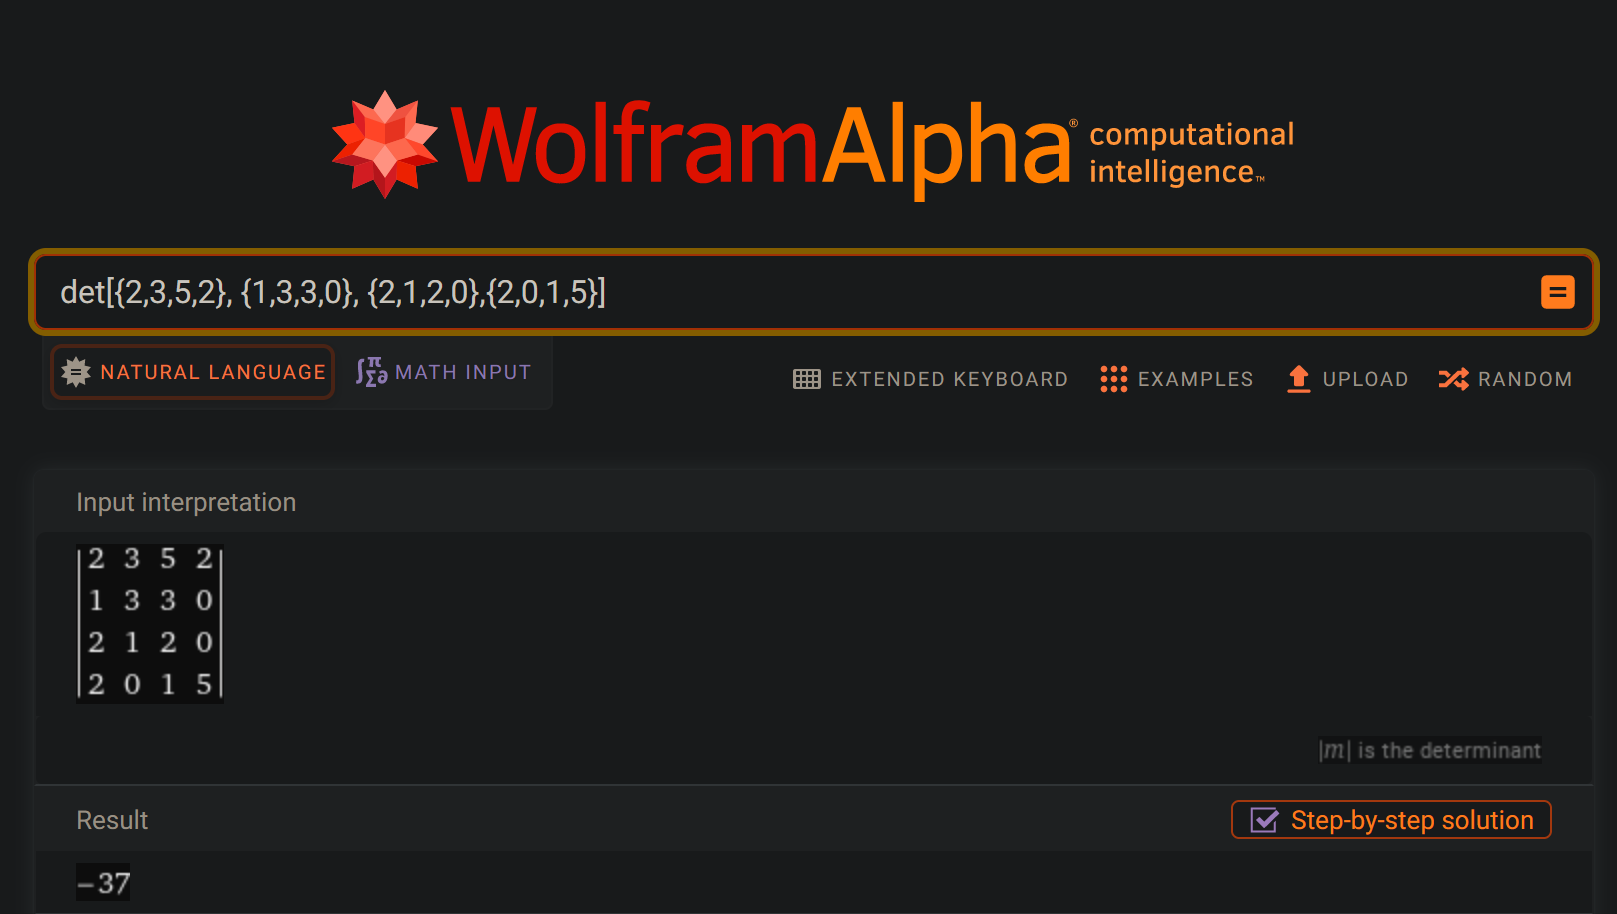
\includegraphics[width=\textwidth]{1}

\clearpage

\section*{2. Uzdevums}
a) Aprēķiniet 5-dimensiju vektoru \{2,-3,5,6,-1\}, \{-1,2,2,-3,1\} skalāro reizinājumu. b) Sareiziniet matricu [\{1,-2,3\},\{4,-5,6\},\{0,8,7\}] ar vertikālo vektoru \{-1,3,2\}.

\begin{gather*}
    \begin{pmatrix}
        2\\
        -3\\
        5\\
        6\\
        -1
    \end{pmatrix}
    \cdot
    \begin{pmatrix}
        -1\\
        2\\
        2\\
        -3\\
        1
    \end{pmatrix}
    =
    \begin{pmatrix}
        2 \cdot (-1)\\
        -3 \cdot 2\\
        5 \cdot 2\\
        6 \cdot (-3)\\
        -1 \cdot 1
    \end{pmatrix}
    =
    (-2 + -6 + 10 + -18 + -1)
    =
    (-17)
\end{gather*}

\begin{gather*}
    \begin{pmatrix}
        1 & -2 & 3\\
        4 & -5 & 6\\
        0 & 8 & 7
    \end{pmatrix}
    \cdot
    \begin{pmatrix}
        -1\\
        3\\
        2
    \end{pmatrix}
    =
    \begin{pmatrix}
        1 \cdot (-1) + (-2) \cdot 3 + 3 \cdot 2\\
        4 \cdot (-1) + (-5) \cdot 3 + 6 \cdot 2\\
        0 \cdot (-1) + 8 \cdot 3 + 7 \cdot 2
    \end{pmatrix}
    =
    \begin{pmatrix}
        -1\\
        9\\
        36
    \end{pmatrix}
\end{gather*}

\clearpage

\section*{3. Uzdevums}
Dotas matricas A=[\{-1,2\},\{3,-5\}], B=[\{1,2\},\{3,4\}], C=[\{1,-2\},\{-3,3\}], . Aprēķiniet reizinājumus AB, BA, (AB)C, A(BC). Pārliecinieties, ka AB$<>$BA un A(BC)=(AB)C. Ko no tā var secināt?

\begin{gather*}
    \begin{pmatrix}
        -1 & 2\\
        3 & -5
    \end{pmatrix}
    \cdot
    \begin{pmatrix}
        1 & 2\\
        3 & 4
    \end{pmatrix}
    =
    \begin{pmatrix}
        -1 \cdot 1 + 2 \cdot 3 & (-1) \cdot 2 + 2 \cdot 4\\
        3 \cdot 1 + (-5) \cdot 3 & 3 \cdot 2 + (-5) \cdot 4
    \end{pmatrix}
    =
    \begin{pmatrix}
        5 & 6\\
        -12 & -14
    \end{pmatrix}
\end{gather*}

\begin{gather*}
    \begin{pmatrix}
        1 & 2\\
        3 & 4
    \end{pmatrix}
    \cdot
    \begin{pmatrix}
        -1 & 2\\
        3 & -5
    \end{pmatrix}
    =
    \begin{pmatrix}
        1 \cdot (-1) + 2 \cdot 3 & 1 \cdot 2 + 2 \cdot (-5)\\
        3 \cdot (-1) + 4 \cdot 3 & 3 \cdot 2 + 4 \cdot (-5)
    \end{pmatrix}
    =
    \begin{pmatrix}
        5 & -8\\
        9 & -14
    \end{pmatrix}
\end{gather*}
    
\begin{equation*}
    \begin{pmatrix}
        5 & 6\\
        -12 & -14
    \end{pmatrix}
    \ne
    \begin{pmatrix}
        5 & -8\\
        9 & -14
    \end{pmatrix}
\end{equation*}

\begin{gather*}
    \left(
        \begin{pmatrix}
            -1 & 2\\
            3 & -5
        \end{pmatrix}
        \cdot
        \begin{pmatrix}
            1 & 2\\
            3 & 4
        \end{pmatrix}
    \right)
    \cdot
    \begin{pmatrix}
        1 & -2\\
        -3 & 3
    \end{pmatrix}
    =
    \begin{pmatrix}
        5 & 6\\
        -12 & -14
    \end{pmatrix}
    \cdot
    \begin{pmatrix}
        1 & -2\\
        -3 & 3
    \end{pmatrix}
    =
    \\
    =
    \begin{pmatrix}
        5 \cdot 1 + 6 \cdot (-3) & 5 \cdot (-2) + 6 \cdot 3\\
        (-12) \cdot 1 + (-14) \cdot (-3) & (-12) \cdot (-2) + (-14) \cdot 3
    \end{pmatrix}
    =
    \begin{pmatrix}
        -13 & 8\\
        30 & -18
    \end{pmatrix}
\end{gather*}

\begin{gather*}
    \begin{pmatrix}
        -1 & 2\\
        3 & -5
    \end{pmatrix}
    \cdot
    \left(
        \begin{pmatrix}
            1 & 2\\
            3 & 4
        \end{pmatrix}
        \cdot
        \begin{pmatrix}
            1 & -2\\
            -3 & 3
        \end{pmatrix}
    \right)
    =
    \\
    =
    \begin{pmatrix}
        -1 & 2\\
        3 & -5
    \end{pmatrix}
    \cdot
    \begin{pmatrix}
        -5 & 4\\
        -9 & 6
    \end{pmatrix}
    =
    \begin{pmatrix}
        -13 & 8\\
        30 & -18
    \end{pmatrix}
\end{gather*}

\begin{equation*}
    \begin{pmatrix}
        -13 & 8\\
        30 & -18
    \end{pmatrix}
    =
    \begin{pmatrix}
        -13 & 8\\
        30 & -18
    \end{pmatrix}
\end{equation*}

Matricu reizināšana nav komutatīva, bet ir distributīva.

\end{document}